\paragraph{Procesamiento de Audio}

La última página web se encarga de todo el procesamiento de audio. En primer lugar, nos encontramos con la sección llamada \textit{Ecualizador}, el cual nos permite elegir, mediante unos sliders vertiales, entre un rango de valores, la ecualización que se desee aplicar en las diferentes bandas posibles.

A continuación, en la sección denominada \textit{Guardar Conf.}, nos encontramos un botón que nos permite guardar la configuración de los distintos filtros en la tarjeta microSD conectada al sistema.

Por último, de la misma manera que en las dos anteriores páginas, nos encontramos los controles que nos permiten modificar el volumen del sistema y seleccionar la salida de auido.

\begin{figure}[h]
    \centering
    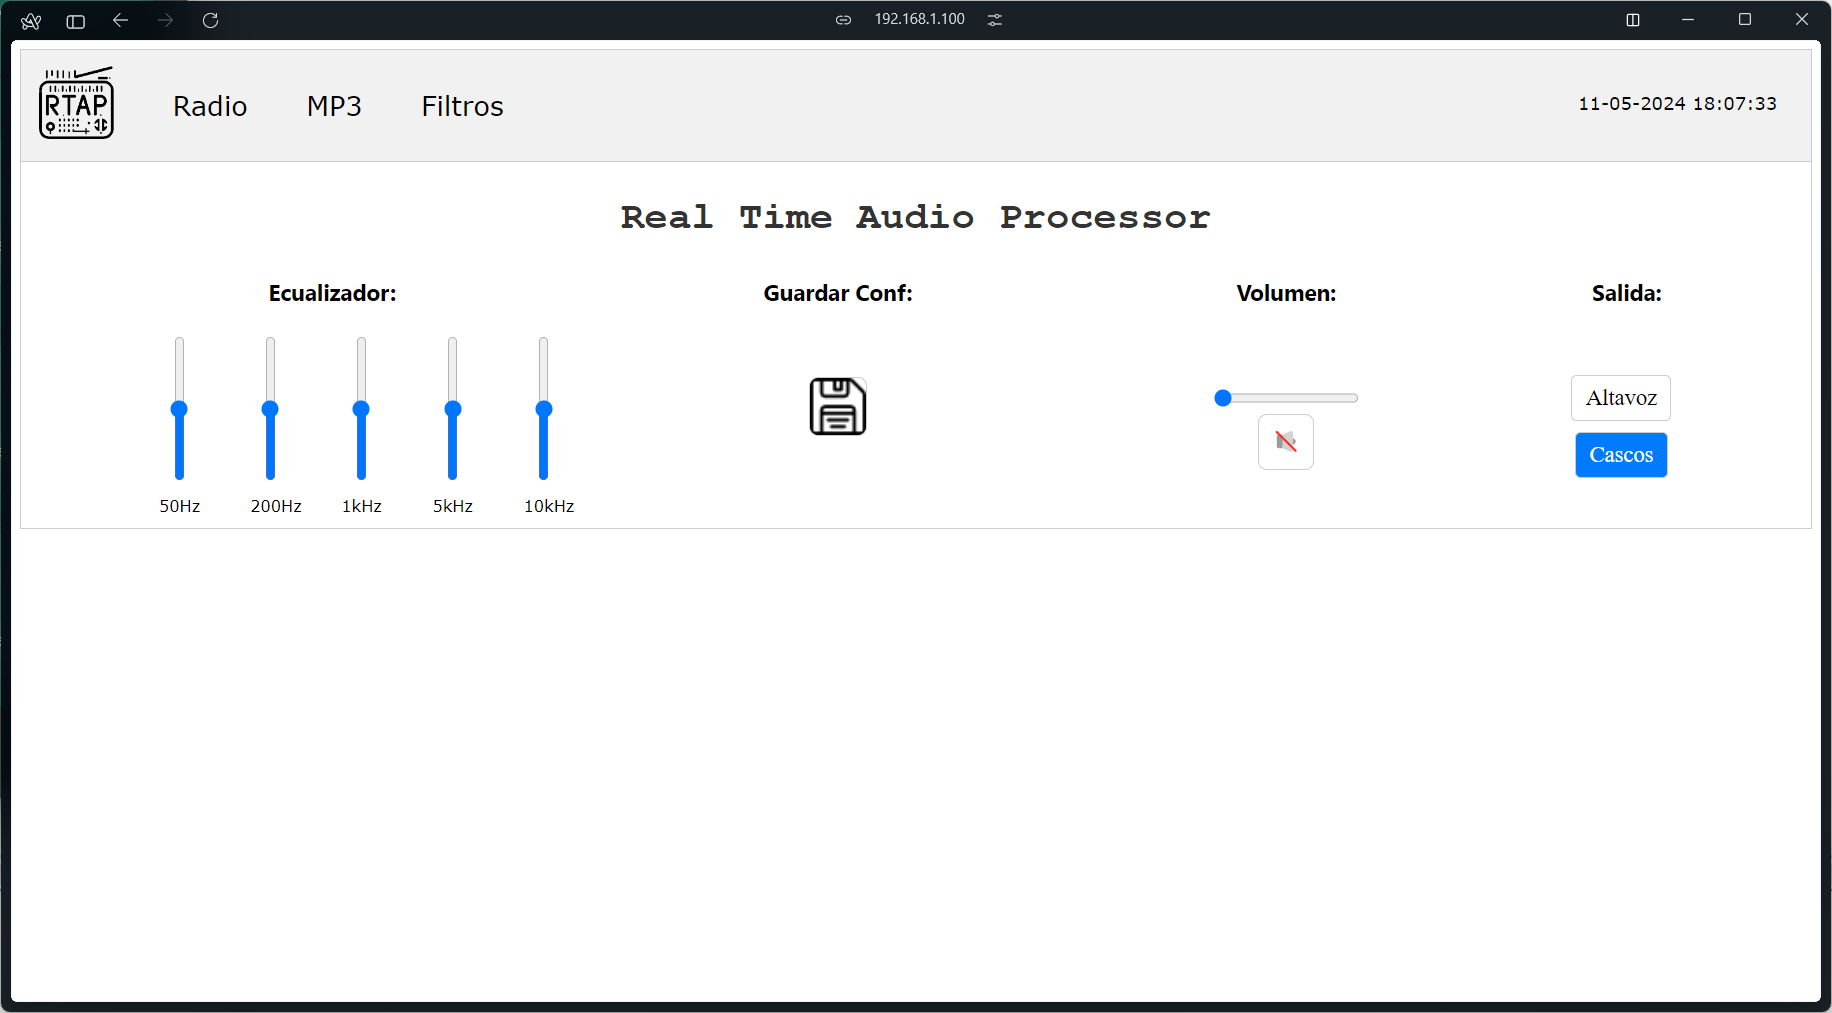
\includegraphics[width=0.8\textwidth]{images/3/3-1/3-1-1-4/Pagina_Filtros.png}
    \caption{Página Filtros}
    \label{fig:3-1-1-4-Filtros}
\end{figure}